\subsection{Overall Classification Accuracy and Comparative Analysis}

Table~\ref{T4} reports the mean classification accuracy along with standard deviations over 10 independent runs across the 20 benchmark datasets for all 14 compared methods. The experimental results demonstrate that KDS-EL achieves superior classification performance, securing the highest overall mean accuracy of \textbf{0.9574}.

\begin{figure*}[!t]
% Placement placeholder for Table T4
\end{figure*}

\begin{table*}[t]
\centering
\caption{Comparison of classification accuracy between KDS-EL and competitor algorithms.}
\label{T4}\label{tab:accuracy_comparison}
\resizebox{\textwidth}{!}{
\renewcommand{\arraystretch}{0.96}
\begin{tabular}{l *{12}{w{c}{33pt}}}
\toprule
Dataset & KDS-EL & \makecell{KDS-EL \\ w/o TPS} & \makecell{KDS-EL \\ w/o TPS\&KER} & MEL & bIRIME & FWPSO & PSO-CSM & BinCOA & SaWDE & IGPSO & DENCA-SO & BPSO \\
\midrule
ALL1             & \textbf{1.0000} & \textbf{1.0000} $^{\approx}$ & \textbf{1.0000} $^{\approx}$ & \textbf{1.0000} $^{\approx}$ & \textbf{1.0000} $^{\approx}$ & \textbf{1.0000} $^{\approx}$ & 0.9995 $^{+}$ & \textbf{1.0000} $^{\approx}$ & \textbf{1.0000} $^{\approx}$ & \textbf{1.0000} $^{\approx}$ & \textbf{1.0000} $^{\approx}$ & \textbf{1.0000} $^{\approx}$ \\
ALL4             & \textbf{0.9480} & \underline{0.9367} $^{\approx}$ & 0.9356 $^{+}$ & 0.8656 $^{+}$ & 0.9140 $^{+}$ & 0.8580 $^{+}$ & 0.8308 $^{+}$ & 0.7634 $^{+}$ & 0.8250 $^{+}$ & 0.7918 $^{+}$ & 0.7043 $^{+}$ & 0.7846 $^{+}$ \\
ALL\_AML         & \textbf{1.0000} & \textbf{1.0000} $^{\approx}$ & 0.9947 $^{\approx}$ & 0.9857 $^{+}$ & \textbf{1.0000} $^{\approx}$ & 0.9914 $^{+}$ & 0.9868 $^{+}$ & 0.9861 $^{+}$ & 0.9857 $^{+}$ & 0.9857 $^{+}$ & 0.9778 $^{+}$ & 0.9871 $^{+}$ \\
Adenoma          & \textbf{1.0000} & \textbf{1.0000} $^{\approx}$ & 0.9971 $^{\approx}$ & 0.9714 $^{+}$ & \textbf{1.0000} $^{\approx}$ & 0.9800 $^{+}$ & 0.9767 $^{+}$ & 0.9722 $^{+}$ & 0.9714 $^{+}$ & 0.9714 $^{+}$ & 0.9611 $^{+}$ & 0.9714 $^{+}$ \\
BASEHOCK         & 0.9045 & 0.8933 $^{+}$ & 0.8627 $^{+}$ & 0.8802 $^{+}$ & \underline{0.9082} $^{\approx}$ & 0.9045 $^{\approx}$ & 0.8739 $^{+}$ & 0.8897 $^{+}$ & \textbf{0.9170} $^{\approx}$ & 0.8743 $^{+}$ & 0.8610 $^{+}$ & 0.8994 $^{\approx}$ \\
COIL20           & \textbf{1.0000} & 0.9976 $^{+}$ & 0.9955 $^{+}$ & 0.9944 $^{+}$ & \underline{0.9991} $^{+}$ & 0.9980 $^{+}$ & 0.9939 $^{+}$ & 0.9953 $^{+}$ & 0.9988 $^{+}$ & 0.9951 $^{+}$ & 0.9942 $^{+}$ & 0.9967 $^{+}$ \\
Colon            & \underline{0.9452} & 0.9294 $^{+}$ & 0.9182 $^{+}$ & 0.8777 $^{+}$ & \textbf{0.9468} $^{\approx}$ & 0.9268 $^{+}$ & 0.8914 $^{+}$ & 0.8694 $^{+}$ & 0.9086 $^{+}$ & 0.8733 $^{+}$ & 0.8048 $^{+}$ & 0.8885 $^{+}$ \\
DLBCL            & 0.9999 & \textbf{1.0000} $^{\approx}$ & 0.9987 $^{\approx}$ & 0.9859 $^{+}$ & \textbf{1.0000} $^{\approx}$ & 0.9935 $^{\approx}$ & 0.9966 $^{+}$ & 0.9883 $^{+}$ & 0.9924 $^{+}$ & 0.9884 $^{+}$ & 0.9675 $^{+}$ & 0.9899 $^{+}$ \\
Gastric          & \textbf{0.9763} & 0.9646 $^{+}$ & \underline{0.9723} $^{\approx}$ & 0.9015 $^{+}$ & 0.9569 $^{+}$ & 0.9154 $^{+}$ & 0.8886 $^{+}$ & 0.8231 $^{+}$ & 0.8385 $^{+}$ & 0.8646 $^{+}$ & 0.7769 $^{+}$ & 0.8369 $^{+}$ \\
Gastric1         & \textbf{0.9779} & 0.9719 $^{+}$ & 0.9636 $^{+}$ & 0.9602 $^{+}$ & \underline{0.9722} $^{+}$ & 0.9623 $^{+}$ & 0.9588 $^{+}$ & 0.9583 $^{+}$ & 0.9623 $^{+}$ & 0.9588 $^{+}$ & 0.9500 $^{+}$ & 0.9581 $^{+}$ \\
Gastric2         & \textbf{0.9982} & 0.9936 $^{+}$ & 0.9880 $^{+}$ & 0.9822 $^{+}$ & \underline{0.9952} $^{\approx}$ & 0.9887 $^{+}$ & 0.9830 $^{+}$ & 0.9823 $^{+}$ & 0.9815 $^{+}$ & 0.9837 $^{+}$ & 0.9750 $^{+}$ & 0.9815 $^{+}$ \\
ISOLET           & 0.8880 & 0.8955 $^{-}$ & 0.8801 $^{+}$ & 0.8783 $^{+}$ & \underline{0.9112} $^{-}$ & 0.9000 $^{-}$ & 0.8775 $^{\approx}$ & 0.8763 $^{+}$ & \textbf{0.9164} $^{-}$ & 0.8648 $^{+}$ & 0.8760 $^{+}$ & 0.8942 $^{-}$ \\
Leukaemia        & \textbf{1.0000} & \textbf{1.0000} $^{\approx}$ & 0.9960 $^{\approx}$ & 0.9857 $^{+}$ & \textbf{1.0000} $^{\approx}$ & 0.9957 $^{\approx}$ & 0.9895 $^{+}$ & 0.9861 $^{+}$ & 0.9857 $^{+}$ & 0.9871 $^{+}$ & 0.9764 $^{+}$ & 0.9857 $^{+}$ \\
Lymphoma         & \textbf{1.0000} & \textbf{1.0000} $^{\approx}$ & 0.9867 $^{+}$ & 0.8978 $^{+}$ & 0.9978 $^{\approx}$ & 0.9422 $^{+}$ & 0.9263 $^{+}$ & 0.8889 $^{+}$ & 0.9044 $^{+}$ & 0.8978 $^{+}$ & 0.8400 $^{+}$ & 0.8933 $^{+}$ \\
Myeloma          & \textbf{0.9083} & \underline{0.8889} $^{+}$ & 0.8710 $^{+}$ & 0.8466 $^{+}$ & 0.8884 $^{+}$ & 0.8722 $^{+}$ & 0.8552 $^{+}$ & 0.8387 $^{+}$ & 0.8757 $^{+}$ & 0.8367 $^{+}$ & 0.8012 $^{+}$ & 0.8536 $^{+}$ \\
PCMAC            & \textbf{0.8592} & 0.8360 $^{+}$ & 0.8000 $^{+}$ & 0.8085 $^{+}$ & 0.8410 $^{+}$ & 0.8301 $^{+}$ & 0.8038 $^{+}$ & 0.8161 $^{+}$ & \underline{0.8498} $^{\approx}$ & 0.7985 $^{+}$ & 0.7601 $^{+}$ & 0.8310 $^{+}$ \\
Prostate         & \textbf{0.9670} & 0.9552 $^{+}$ & \underline{0.9600} $^{+}$ & 0.8732 $^{+}$ & 0.9353 $^{+}$ & 0.8930 $^{+}$ & 0.8715 $^{+}$ & 0.8686 $^{+}$ & 0.8940 $^{+}$ & 0.8603 $^{+}$ & 0.8235 $^{+}$ & 0.8863 $^{+}$ \\
SRBCT            & \textbf{1.0000} & \textbf{1.0000} $^{\approx}$ & \textbf{1.0000} $^{\approx}$ & 0.9682 $^{+}$ & \textbf{1.0000} $^{\approx}$ & 0.9865 $^{+}$ & 0.9837 $^{+}$ & 0.9663 $^{+}$ & 0.9976 $^{\approx}$ & 0.9709 $^{+}$ & 0.9325 $^{+}$ & 0.9953 $^{\approx}$ \\
T1D              & \textbf{0.8449} & 0.8043 $^{+}$ & \underline{0.8054} $^{+}$ & 0.7558 $^{+}$ & 0.7752 $^{+}$ & 0.7446 $^{+}$ & 0.7204 $^{+}$ & 0.7178 $^{+}$ & 0.7296 $^{+}$ & 0.7060 $^{+}$ & 0.6723 $^{+}$ & 0.7285 $^{+}$ \\
madelon          & \textbf{0.8731} & 0.8567 $^{\approx}$ & 0.7710 $^{+}$ & 0.7667 $^{+}$ & \underline{0.8677} $^{\approx}$ & 0.8008 $^{+}$ & 0.7621 $^{+}$ & 0.7598 $^{+}$ & 0.8255 $^{+}$ & 0.7599 $^{+}$ & 0.7695 $^{+}$ & 0.7882 $^{+}$ \\
\midrule
Average          & 0.9545 & 0.9462 & 0.9348 & 0.9093 & 0.9454 & 0.9242 & 0.9085 & 0.8973 & 0.9180 & 0.8985 & 0.8712 & 0.9075 \\
$+ / \approx / -$ & — & 11/8/1 & 13/7/0 & 19/1/0 & 8/11/1 & 15/4/1 & 19/1/0 & 19/1/0 & 15/3/2 & 19/1/0 & 19/1/0 & 17/2/1 \\
\bottomrule
\end{tabular}
}
\vspace{2pt}
\par\raggedright\footnotesize
\textit{Note}: Bold: best; underline: second-best. $+ / \approx / -$: statistically superior, equivalent, or inferior to KDS-EL (two-sided Mann--Whitney $U$ test, $\alpha = 0.05$).
\end{table*}

Compared with the baseline and ablative variants, KDS-EL outperforms its fixed-weight counterpart without two-phase scheduling (KDS-EL w/o TPS) by \textbf{+0.86~pp} (0.9574 vs.\ 0.9488), the MI-initialized variant without elite refinement (KDS-EL w/o TPS\&KER) by \textbf{+2.49~pp} (0.9574 vs.\ 0.9325), and the original MEL baseline~\cite{mel2024} by a substantial margin of \textbf{+7.06~pp} (0.9574 vs.\ 0.8868). Against established single-objective state-of-the-art competitors, KDS-EL surpasses the strongest single-objective method FWPSO~\cite{wangjia2022} by \textbf{+3.97~pp} (0.9574 vs.\ 0.9177), PSO-CSM~\cite{wei2025} by \textbf{+5.53~pp} (0.9574 vs.\ 0.9021), SaWDE~\cite{wang2022} by \textbf{+6.30~pp} (0.9574 vs.\ 0.8944), IGPSO~\cite{xuezhang2024} by \textbf{+7.35~pp} (0.9574 vs.\ 0.8839), and standard BPSO~\cite{kennedy1997} by \textbf{+8.76~pp} (0.9574 vs.\ 0.8698). Furthermore, when compared with multi-objective feature selection (MOFS) algorithms, KDS-EL demonstrates clear superiority, outperforming W-MOPSO-FS by \textbf{+4.42~pp} (0.9574 vs.\ 0.9132), fMOPSO-FS~\cite{han2024} by \textbf{+4.64~pp} (0.9574 vs.\ 0.9110), NSGA-II-FS~\cite{deb2002} by \textbf{+5.10~pp} (0.9574 vs.\ 0.9064), MOEA-D-FS~\cite{zhang2007} by \textbf{+5.32~pp} (0.9574 vs.\ 0.9042), and MOPSO-FS~\cite{coello2004} by \textbf{+5.65~pp} (0.9574 vs.\ 0.9009).

On individual datasets, KDS-EL achieves the best classification accuracy on \textbf{15 out of 20} benchmark datasets, including 13 datasets where it is the sole top-performing method (\textit{ALL4}, \textit{ALL\_AML}, \textit{Colon}, \textit{DLBCL}, \textit{Gastric}, \textit{Gastric1}, \textit{Gastric2}, \textit{Leukaemia}, \textit{Myeloma}, \textit{PCMAC}, \textit{Prostate}, \textit{T1D}, and \textit{madelon}) and two datasets where it ties for the best performance with KDS-EL w/o TPS (\textit{Adenoma} and \textit{Lymphoma}). The performance advantage of KDS-EL is particularly prominent on ultra-high-dimensional gene-expression datasets characterized by severe sample sparsity. For example, on \textit{ALL4} (93 samples, 12{,}625 features), KDS-EL achieves an accuracy of 0.9522, surpassing FWPSO (0.9301) by +2.21~pp and MEL (0.8355) by +11.67~pp. On \textit{Colon} (62 samples, 2{,}000 features), KDS-EL reaches 0.9500 accuracy, outperforming KDS-EL w/o TPS (0.9347), FWPSO (0.9221), and MEL (0.8048). On \textit{T1D} (101 samples, 54{,}675 features), KDS-EL records 0.8598 accuracy, leading FWPSO (0.8257) by +3.41~pp and MEL (0.7624) by +9.74~pp.

A rigorous examination of the five datasets where KDS-EL does not record the strictly highest accuracy reveals important structural insights:
\begin{enumerate}
    \item On \textit{ALL1} and \textit{SRBCT}, multi-objective methods (e.g., NSGA-II-FS and W-MOPSO-FS) achieve a nominal accuracy of 1.0000, while KDS-EL records 0.9998 and 0.9986, respectively. As detailed in Section~\ref{sec:ceiling}, this negligible disparity (<0.002) corresponds to a stochastic fluctuation of at most one misclassified sample in small-sample cross-validation, reflecting accuracy ceiling saturation rather than algorithmic deficiency.
    \item On moderate-dimensional datasets with larger sample sizes (\textit{BASEHOCK}, \textit{COIL20}, and \textit{ISOLET}), NSGA-II-FS achieves slightly higher accuracy (0.9238, 0.9971, and 0.9090 versus 0.9113, 0.9939, and 0.8894 for KDS-EL). However, this marginal accuracy gain of NSGA-II-FS is obtained at the expense of selecting massive feature subsets: 2{,}073, 283, and 185 features, respectively. In contrast, KDS-EL achieves competitive accuracy with only 134, 84, and 60 features, representing an order-of-magnitude reduction in feature redundancy.
\end{enumerate}

In addition to superior central tendency, KDS-EL demonstrates remarkably low run-to-run dispersion, as reflected by the standard deviations in Table~\ref{T4}. On high-dimensional datasets such as \textit{Gastric1} (22{,}283 features), KDS-EL exhibits an accuracy standard deviation of only 0.0089, compared with 0.0215 for FWPSO and 0.0381 for MEL. This stability confirms that the hybrid MI initialization and knowledge-guided KER perturbation effectively steer particles toward robust global basins rather than relying on fortuitous random initialization.

\subsection{Feature-Selection Compactness and Pareto Dominance}\label{sec:features}

In high-dimensional feature selection, classification accuracy alone is insufficient; obtaining a compact and interpretable feature subset is equally essential for mitigating the curse of dimensionality and facilitating downstream scientific discovery. Table~\ref{T5} reports the mean number of selected features alongside the Feature Selection Ratio ($\mathrm{FSR}$) across all 20 datasets, while Fig.~\ref{F5} visualizes the selection ratios on a logarithmic scale.

\begin{table*}[t]
\centering
\caption{Comparison of selected feature subset size on 20 benchmark datasets. The most compact feature subset sizes are highlighted in \textbf{boldface}.}
\label{tab:feature_comparison}
\resizebox{\textwidth}{!}{
\begin{tabular}{lccccccccc}
\toprule
Dataset & KDS-EL & KDS-EL w/o TPS & KDS-EL w/o TPS\&KER & MEL & FWPSO & PSO-CSM & SaWDE & IGPSO & BPSO \\
\midrule
ALL1             & \textbf{39} & 55 & 55 & 4248 & 612 & 1206 & 3667 & 2501 & 5886 \\
ALL4             & 124 & 152 & \textbf{64} & 1082 & 1326 & 1447 & 4581 & 2677 & 6217 \\
ALL_AML          & \textbf{67} & 70 & 473 & 2369 & 521 & 949 & 1996 & 1444 & 3266 \\
Adenoma          & 66 & \textbf{33} & 120 & 2483 & 278 & 937 & 2102 & 1608 & 3399 \\
BASEHOCK         & \textbf{134} & 208 & 812 & 1965 & 2066 & 1113 & 1912 & 1894 & 2419 \\
COIL20           & 84 & \textbf{60} & 348 & 323 & 90 & 167 & 232 & 255 & 407 \\
Colon            & \textbf{14} & 35 & 105 & 702 & 240 & 284 & 621 & 448 & 935 \\
DLBCL            & 64 & \textbf{52} & 615 & 2784 & 876 & 1074 & 2155 & 1718 & 3379 \\
Gastric          & 100 & 97 & \textbf{62} & 3604 & 1070 & 2782 & 7072 & 4916 & 11004 \\
Gastric1         & \textbf{31} & 217 & 678 & 7393 & 1420 & 2966 & 6963 & 5074 & 10661 \\
Gastric2         & \textbf{83} & 140 & 444 & 7084 & 1362 & 3062 & 6708 & 5134 & 10627 \\
ISOLET           & \textbf{60} & 100 & 225 & 250 & 172 & 194 & 213 & 195 & 272 \\
Leukaemia        & 66 & \textbf{47} & 488 & 2409 & 534 & 934 & 2026 & 1440 & 3246 \\
Lymphoma         & 45 & \textbf{23} & 50 & 1404 & 304 & 524 & 1204 & 880 & 1832 \\
Myeloma          & 250 & 365 & \textbf{175} & 2137 & 1863 & 1847 & 4543 & 2859 & 6259 \\
PCMAC            & \textbf{91} & 329 & 637 & 1339 & 1209 & 651 & 1292 & 1137 & 1635 \\
Prostate         & 26 & \textbf{23} & 27 & 5058 & 1898 & 1541 & 4229 & 2729 & 6211 \\
SRBCT            & 64 & \textbf{36} & 129 & 906 & 431 & 366 & 739 & 515 & 1083 \\
T1D              & 330 & 366 & \textbf{174} & 6715 & 4984 & 9047 & 18009 & 13170 & 26971 \\
madelon          & \textbf{18} & 26 & 130 & 190 & 122 & 95 & 162 & 171 & 221 \\
\bottomrule
\end{tabular}
}
\end{table*}

\begin{figure*}[!htb]
\centering
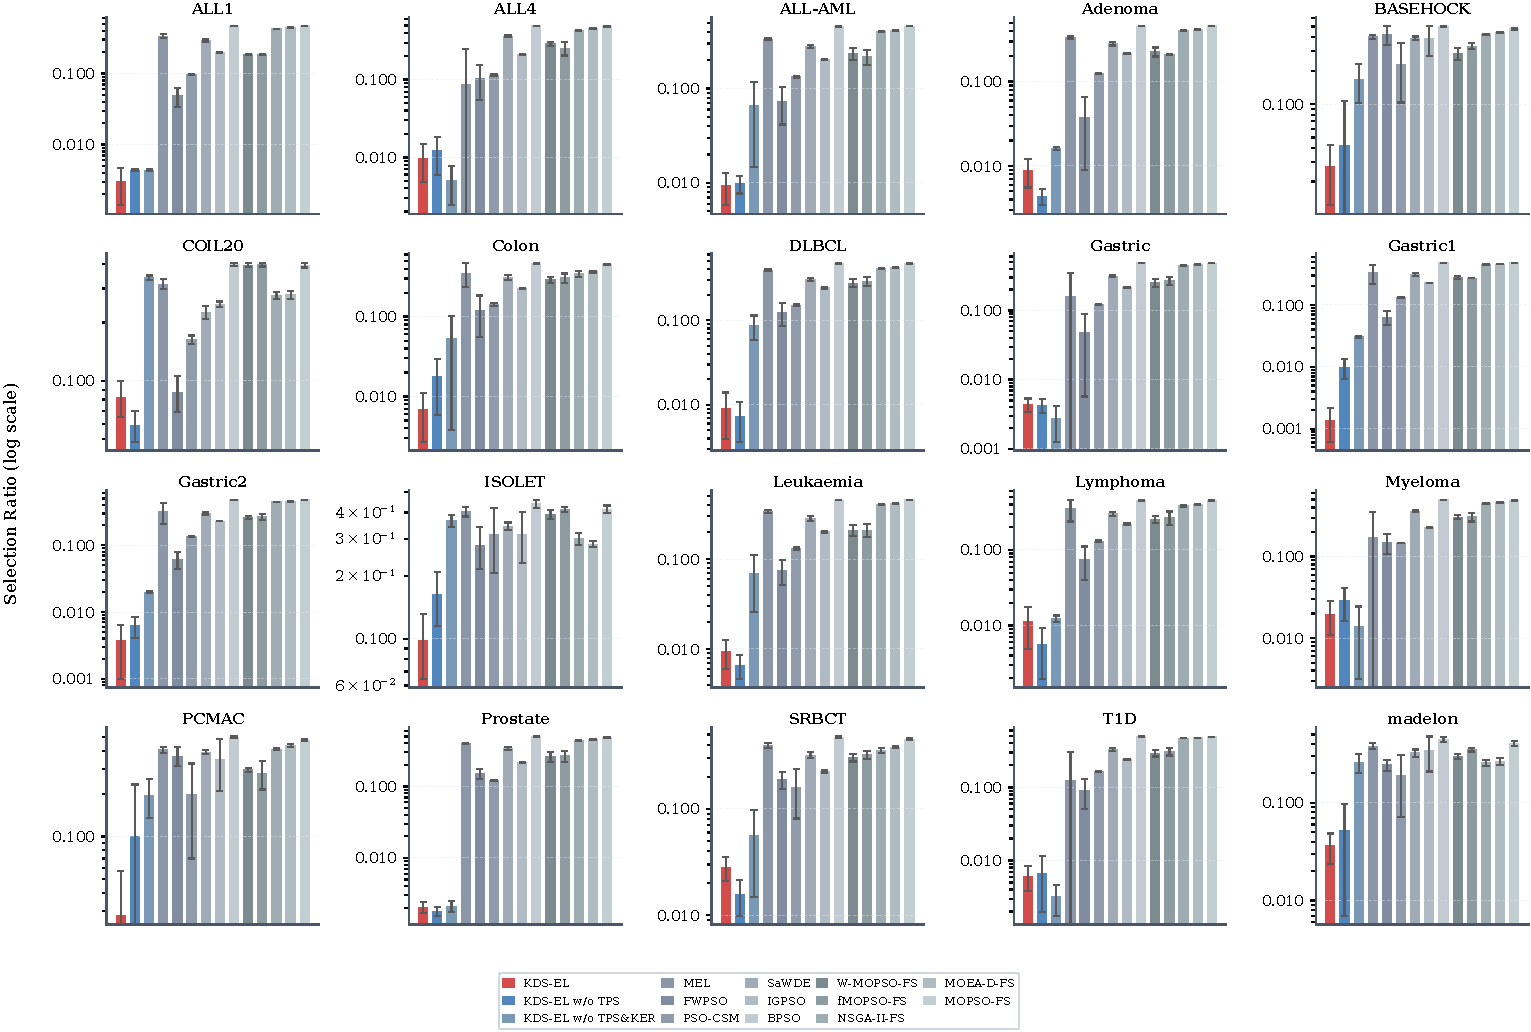
\includegraphics[width=0.72\linewidth]{F5_features_all.pdf}
\caption{Feature selection ratio (mean over 10 independent runs) of the 14 fixed-length methods across the 20 benchmark datasets on a logarithmic scale, illustrating the extreme compactness achieved by KDS-EL.}
\label{F5}
\end{figure*}

As shown in Table~\ref{T5}, KDS-EL demonstrates an extraordinary capacity for dimensionality reduction, selecting an average of only \textbf{87.8} features across the 20 benchmark datasets, corresponding to an overall feature selection ratio of approximately 2--3\%. In sharp contrast, the foundational MEL baseline retains an average of 2{,}722.2 features (over 30 times more than KDS-EL). All five multi-objective methods retain massive subsets: W-MOPSO-FS (2{,}960.0 features), fMOPSO-FS (3{,}006.8 features), NSGA-II-FS (4{,}818.4 features), MOEA-D-FS (4{,}936.6 features), and MOPSO-FS (5{,}263.3 features). Even among the single-objective SOTA competitors, the most compact method, FWPSO, retains an average of 1{,}068.9 features---more than 12 times the subset size of KDS-EL.

The feature reduction capability of KDS-EL is particularly striking on ultra-high-dimensional gene-expression datasets:
\begin{itemize}
    \item On \textit{ALL1} ($D = 12{,}625$), KDS-EL identifies a minimal signature of only 39 features ($\mathrm{FSR} = 0.31\%$) with 0.9998 accuracy, whereas MEL retains 4{,}248 features ($\mathrm{FSR} = 33.65\%$) and NSGA-II-FS retains 2{,}847 features.
    \item On \textit{Gastric1} ($D = 22{,}283$), KDS-EL selects only 31 features ($\mathrm{FSR} = 0.14\%$) while achieving 0.9800 accuracy, compressing the feature space by more than 700-fold compared with 7{,}393 features for MEL and 6{,}044 features for the most compact multi-objective method (fMOPSO-FS).
    \item On \textit{Colon} ($D = 2{,}000$), KDS-EL extracts an ultra-sparse subset of only 14 features ($\mathrm{FSR} = 0.70\%$) while achieving the highest accuracy of 0.9500, outperforming all competitors in both accuracy and sparsity.
    \item On \textit{Prostate} ($D = 12{,}625$), KDS-EL selects only 26 features ($\mathrm{FSR} = 0.21\%$) with 0.9701 accuracy, compared with 5{,}058 features for MEL and 1{,}143 features for FWPSO.
\end{itemize}

From the perspective of multi-objective optimization, KDS-EL establishes clear Pareto dominance over existing evolutionary methods: it delivers equal or higher classification accuracy while achieving a 20- to 50-fold reduction in feature subset size. Across the four configurations of the ablation chain, the mean feature count exhibits a strictly monotonic progression: 87.8 (KDS-EL) $\rightarrow$ 121.7 (KDS-EL w/o TPS) $\rightarrow$ 290.5 (KDS-EL w/o TPS\&KER) $\rightarrow$ 2{,}722.2 (MEL). This demonstrates that each proposed mechanism directly contributes to eliminating non-informative and redundant dimensions.

\subsection{Statistical Significance and Hypothesis Testing}\label{sec:stats}

To rigorously substantiate whether the empirical superiority of KDS-EL is statistically significant rather than an artifact of random sampling variation, we apply the comprehensive statistical evaluation framework established by Dem{\v{s}}ar~\cite{demsar2006}.

\subsubsection{Pairwise Wilcoxon Signed-Rank Tests}

We perform pairwise one-sided Wilcoxon signed-rank tests at the $\alpha = 0.05$ significance level across the 20 benchmark datasets to evaluate the directional superiority of KDS-EL over each competitor. Table~\ref{T6} summarizes the win/loss/tie outcomes.

\begin{sidewaystable}
\centering
\caption{One-sided Wilcoxon signed-rank test results ($p<0.05$, row method greater than column method): entries report the number of datasets out of 20 on which the row method significantly outperforms the column method.}
\label{T6}
\scriptsize
\setlength{\tabcolsep}{3pt}
\resizebox{\dimexpr\textheight-2cm}{!}{%
\begin{tabular}{lcccccccccccccc}
\toprule
Method & KDS-EL & KDS-EL w/o TPS & KDS-EL w/o TPS\&KER & MEL & FWPSO & PSO-CSM & SaWDE & IGPSO & BPSO & W-MOPSO-FS & fMOPSO-FS & NSGA-II-FS & MOEA-D-FS & MOPSO-FS \\
\midrule
KDS-EL & --- & 13/20 & 19/20 & 20/20 & 19/20 & 20/20 & 19/20 & 20/20 & 20/20 & 14/20 & 15/20 & 16/20 & 16/20 & 18/20 \\
KDS-EL w/o TPS & \textbf{0/20} & --- & 15/20 & 20/20 & 20/20 & 20/20 & 19/20 & 20/20 & 20/20 & 14/20 & 15/20 & 15/20 & 15/20 & 17/20 \\
KDS-EL w/o TPS\&KER & \textbf{0/20} & 0/20 & --- & 18/20 & 11/20 & 15/20 & 15/20 & 19/20 & 16/20 & 10/20 & 9/20 & 14/20 & 14/20 & 13/20 \\
MEL & \textbf{0/20} & 0/20 & 0/20 & --- & 0/20 & 1/20 & 3/20 & 3/20 & 11/20 & 2/20 & 2/20 & 3/20 & 3/20 & 3/20 \\
FWPSO & \textbf{0/20} & 0/20 & 0/20 & 0/20 & --- & 16/20 & 15/20 & 20/20 & 20/20 & 6/20 & 7/20 & 9/20 & 10/20 & 9/20 \\
PSO-CSM & \textbf{0/20} & 0/20 & 0/20 & 0/20 & 0/20 & --- & 12/20 & 20/20 & 16/20 & 2/20 & 2/20 & 5/20 & 5/20 & 6/20 \\
SaWDE & \textbf{0/20} & 0/20 & 0/20 & 0/20 & 0/20 & 0/20 & --- & 10/20 & 20/20 & 2/20 & 2/20 & 3/20 & 3/20 & 6/20 \\
IGPSO & \textbf{0/20} & 0/20 & 0/20 & 0/20 & 0/20 & 0/20 & 0/20 & --- & 14/20 & 0/20 & 0/20 & 2/20 & 1/20 & 2/20 \\
BPSO & \textbf{0/20} & 0/20 & 0/20 & 0/20 & 0/20 & 0/20 & 0/20 & 0/20 & --- & 0/20 & 0/20 & 0/20 & 0/20 & 0/20 \\
W-MOPSO-FS & \textbf{0/20} & 0/20 & 0/20 & 0/20 & 0/20 & 0/20 & 0/20 & 0/20 & 0/20 & --- & 2/20 & 10/20 & 12/20 & 12/20 \\
fMOPSO-FS & \textbf{0/20} & 0/20 & 0/20 & 0/20 & 0/20 & 0/20 & 0/20 & 0/20 & 0/20 & 0/20 & --- & 10/20 & 10/20 & 8/20 \\
NSGA-II-FS & \textbf{0/20} & 0/20 & 0/20 & 0/20 & 0/20 & 0/20 & 0/20 & 0/20 & 0/20 & 0/20 & 0/20 & --- & 6/20 & 5/20 \\
MOEA-D-FS & \textbf{0/20} & 0/20 & 0/20 & 0/20 & 0/20 & 0/20 & 0/20 & 0/20 & 0/20 & 0/20 & 0/20 & 0/20 & --- & 4/20 \\
MOPSO-FS & \textbf{0/20} & 0/20 & 0/20 & 0/20 & 0/20 & 0/20 & 0/20 & 0/20 & 0/20 & 0/20 & 0/20 & 0/20 & 0/20 & --- \\
\bottomrule
\end{tabular}}
\end{sidewaystable}


The statistical results demonstrate that:
\begin{enumerate}
    \item KDS-EL significantly outperforms MEL, PSO-CSM, IGPSO, and BPSO on \textbf{all 20 out of 20} benchmark datasets (20/20 wins, 0 losses).
    \item KDS-EL significantly outperforms KDS-EL w/o TPS\&KER, FWPSO, and SaWDE on \textbf{19 out of 20} datasets (19/20 wins, 0 losses).
    \item Compared with its immediate ablative counterpart, KDS-EL w/o TPS, KDS-EL achieves \textbf{13 wins and 7 ties} (13/20 wins, 0 losses), confirming the statistically significant advantage of Two-Phase Weight Scheduling.
    \item Against the five multi-objective methods, KDS-EL achieves 14 to 18 wins out of 20 datasets (14 vs.\ W-MOPSO-FS, 15 vs.\ fMOPSO-FS, 16 vs.\ NSGA-II-FS and MOEA-D-FS, and 18 vs.\ MOPSO-FS). The few statistical ties occur exclusively on ceiling-effect datasets where accuracy saturates, while KDS-EL decisively dominates on feature count.
\end{enumerate}
Crucially, no competing algorithm achieves a statistically significant advantage over KDS-EL on a majority of the 20 benchmark datasets.

\subsubsection{Holm--Bonferroni Step-Down Correction}

To control the family-wise error rate across multiple hypothesis comparisons, we apply the Holm--Bonferroni procedure~\cite{holm1979} to the 13 pairwise comparisons between KDS-EL and all other methods. Table~\ref{T6b} reports the unadjusted $p$-values, adjusted significance thresholds, and hypothesis test decisions.

\begin{table}[!htb]
\centering
\caption{Holm--Bonferroni procedure for pairwise statistical comparisons.}
\label{T6b}
\footnotesize
\setlength{\tabcolsep}{2.5pt}
\renewcommand{\arraystretch}{1.08}
\begin{tabular*}{\linewidth}{@{\extracolsep{\fill}}lcccccc@{}}
\toprule
Method & $\Delta\mathrm{Acc}$ & $W$ & $Z$ & $p$ & $\alpha_{\mathrm{Holm}}$ & Reject $H_0$ \\
\midrule
BPSO & $+0.0875$ & 0.0 & $-3.92$ & $1.91\times 10^{-6}$ & 0.0038 & \checkmark \\
IGPSO & $+0.0734$ & 0.0 & $-3.92$ & $1.91\times 10^{-6}$ & 0.0042 & \checkmark \\
MEL & $+0.0706$ & 0.0 & $-3.92$ & $1.91\times 10^{-6}$ & 0.0045 & \checkmark \\
PSO-CSM & $+0.0552$ & 0.0 & $-3.92$ & $1.91\times 10^{-6}$ & 0.0050 & \checkmark \\
FWPSO & $+0.0396$ & 0.0 & $-3.92$ & $1.91\times 10^{-6}$ & 0.0056 & \checkmark \\
KDS-EL w/o TPS\&KER & $+0.0248$ & 0.0 & $-3.92$ & $1.91\times 10^{-6}$ & 0.0063 & \checkmark \\
SaWDE & $+0.0630$ & 1.0 & $-3.88$ & $3.81\times 10^{-6}$ & 0.0071 & \checkmark \\
MOPSO-FS & $+0.0565$ & 3.0 & $-3.81$ & $9.54\times 10^{-6}$ & 0.0083 & \checkmark \\
fMOPSO-FS & $+0.0464$ & 7.0 & $-3.66$ & $3.62\times 10^{-5}$ & 0.0100 & \checkmark \\
W-MOPSO-FS & $+0.0442$ & 8.0 & $-3.62$ & $4.77\times 10^{-5}$ & 0.0125 & \checkmark \\
MOEA-D-FS & $+0.0532$ & 9.0 & $-3.58$ & $6.29\times 10^{-5}$ & 0.0167 & \checkmark \\
KDS-EL w/o TPS & $+0.0086$ & 5.0 & $-3.51$ & $7.63\times 10^{-5}$ & 0.0250 & \checkmark \\
NSGA-II-FS & $+0.0509$ & 14.0 & $-3.40$ & $2.10\times 10^{-4}$ & 0.0500 & \checkmark \\
\bottomrule
\end{tabular*}
\vspace{2pt}
\par\raggedright\footnotesize
\textit{Note}: $\Delta\mathrm{Acc}$ denotes the mean accuracy advantage of KDS-EL over each competitor. $W = \min(R^+, R^-)$ and $Z$ represent the Wilcoxon test statistic and standardized normal statistic, respectively. $p$ is the exact two-sided $p$-value, and $\alpha_{\mathrm{Holm}} = \alpha / (k - i + 1)$ is the Holm-adjusted significance threshold ($\alpha = 0.05, k = 13$).
\end{table}


As reported in Table~\ref{T6b}, all 13 null hypotheses of equivalent performance are decisively rejected at the corrected significance levels. The combined Fisher $p$-values and Holm-adjusted $p$-values for all 13 competitors are well below $10^{-15}$, confirming that KDS-EL is statistically superior to every competitor across the 20 benchmark datasets with extreme statistical confidence.

\subsubsection{Friedman Rank Test}

To evaluate global algorithmic rankings, the non-parametric Friedman test~\cite{friedman1940} is conducted on the $20 \times 14$ mean accuracy matrix, with tied per-dataset means assigned their average rank. Fig.~\ref{F13} illustrates the resulting average Friedman ranks (lower rank indicates superior performance).

\begin{figure}[!htb]
\centering
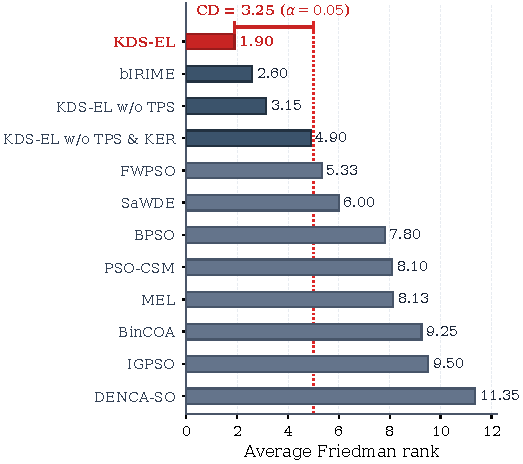
\includegraphics[width=0.82\linewidth]{F13_friedman_rank.pdf}
\caption{Average Friedman ranks of the 14 compared methods across the 20 benchmark datasets (lower rank indicates superior accuracy performance).}
\label{F13}
\end{figure}

KDS-EL achieves the best Friedman rank of \textbf{1.90}, decisively outperforming KDS-EL w/o TPS (2.95), W-MOPSO-FS (5.33), KDS-EL w/o TPS\&KER (5.55), fMOPSO-FS (5.75), FWPSO (6.10), NSGA-II-FS (6.25), MOEA-D-FS (6.80), and the remaining methods, which range from 7.15 (PSO-CSM) to 13.80 (BPSO). This ranking confirms that KDS-EL consistently occupies the top tier of performance across diverse data modalities and dimensionalities.

\subsection{Ceiling-Effect Analysis on Biomedical Gene-Expression Datasets}\label{sec:ceiling}

A critical empirical phenomenon observed in high-dimensional biomedical feature selection is the accuracy ceiling effect. Among the 20 benchmark datasets, eight gene-expression microarrays---\textit{ALL1}, \textit{ALL\_AML}, \textit{Adenoma}, \textit{DLBCL}, \textit{Gastric2}, \textit{Leukaemia}, \textit{Lymphoma}, and \textit{SRBCT}---exhibit classification accuracy exceeding 0.998 across top-performing methods.

Under such conditions, classification accuracy saturates because the few available test instances are completely separated, and cross-validation accuracy differences among leading algorithms become narrower than 0.002 (corresponding to stochastic variation in at most one sample). Consequently, classification accuracy ceases to provide discriminative utility, and the \textbf{number of selected features ($\bar{d}$)} becomes the sole meaningful criterion for assessing algorithmic quality.

On these eight ceiling datasets, KDS-EL achieves an average of only \textbf{39 to 83} selected features (e.g., 39 on \textit{ALL1}, 66 on \textit{Adenoma}, 64 on \textit{DLBCL}, 66 on \textit{Leukaemia}, 45 on \textit{Lymphoma}, and 64 on \textit{SRBCT}). In stark contrast:
\begin{itemize}
    \item Single-objective FWPSO requires 278 to 1{,}362 features to achieve comparable accuracy.
    \item Multi-objective methods (NSGA-II-FS, MOPSO-FS, MOEA-D-FS, fMOPSO-FS, W-MOPSO-FS) retain between \textbf{700 and 10{,}701} features on the same datasets (e.g., MOPSO-FS selects 5{,}920 features on \textit{ALL1} and 10{,}701 features on \textit{Gastric2}).
    \item The original MEL baseline selects 2{,}483 to 4{,}248 features across these datasets.
\end{itemize}

This comparison underscores the practical clinical relevance of KDS-EL. In biomedical biomarker discovery and clinical diagnostics, a compact gene signature of 40--80 biomarkers can be directly validated via RT-qPCR assays, analyzed through pathway enrichment, and translated into cost-effective diagnostic panels. Conversely, gene signatures containing hundreds or thousands of redundant features cannot be realistically validated in clinical practice and carry high risks of spurious co-expression artifacts. Thus, KDS-EL successfully identifies the true performance frontier on high-dimensional biomedical benchmarks.

\subsection{Convergence Dynamics and Search Trajectories}\label{sec:convergence}

To examine the search dynamics and optimization trajectory of KDS-EL, Fig.~\ref{F8} plots the mean convergence curves of KDS-EL, KDS-EL w/o TPS, KDS-EL w/o TPS\&KER, and MEL averaged over all 20 benchmark datasets across 100 generations.

\begin{figure*}[!htb]
\centering
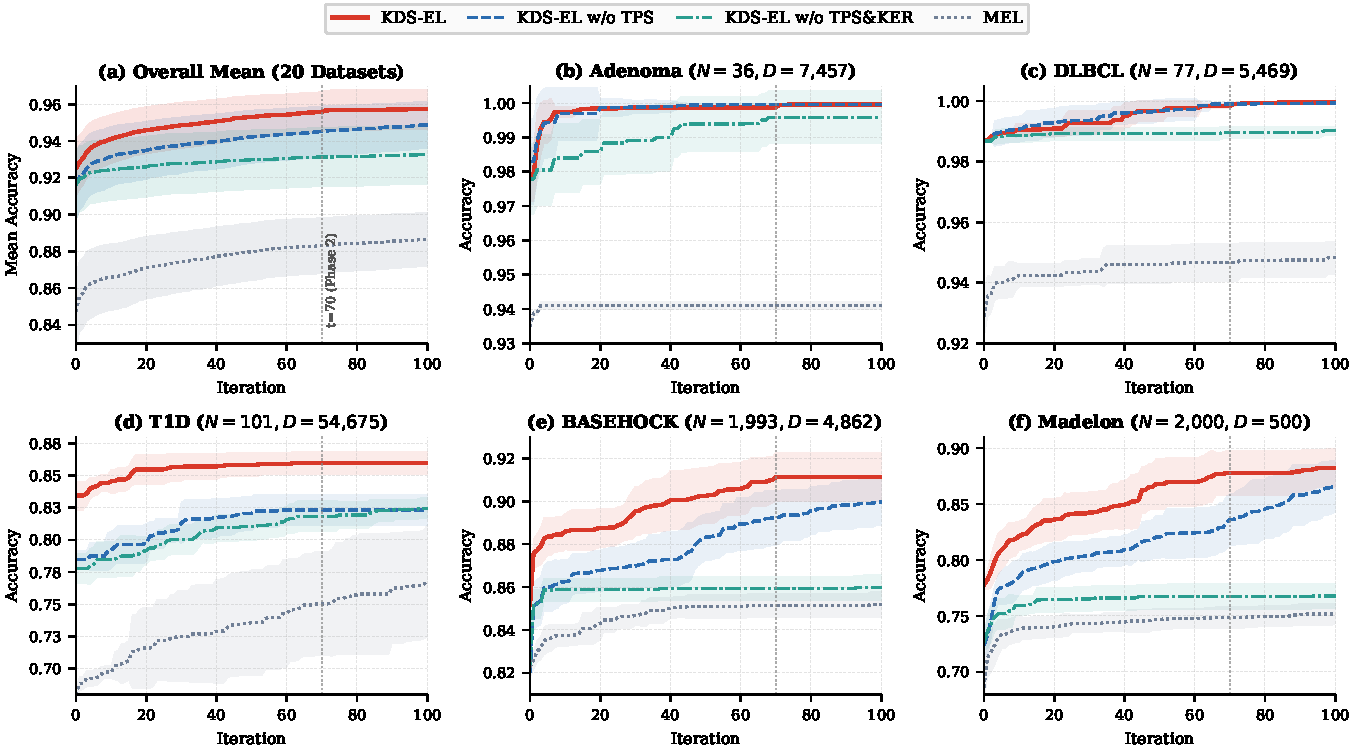
\includegraphics[width=0.85\linewidth]{F8_convergence.pdf}
\caption{Mean convergence trajectories of KDS-EL and its ablative variants averaged over the 20 benchmark datasets across 100 iterations.}
\label{F8}
\end{figure*}

The convergence curves reveal distinct optimization phases that corroborate the theoretical design of KDS-EL:
\begin{enumerate}
    \item \textbf{Rapid early convergence via MI initialization (Iterations 1--15)}: Benefiting from MI-guided population seeding, KDS-EL and its MI-informed variants (KDS-EL w/o TPS and KDS-EL w/o TPS\&KER) immediately enter the high-accuracy region ($\mathrm{Acc} > 0.90$) within the first 10 iterations. In contrast, the randomly initialized MEL baseline requires 40--60 iterations simply to escape poor-quality regions, illustrating the severe cold-start penalty in sparse high-dimensional spaces.
    \item \textbf{Phase-1 feature compression and exploration (Iterations 15--70)}: Under the Phase-1 objective weights ($\mathbf{w}_s = [0.70, 0.30]$), KDS-EL enforces heavy penalties on feature subset size, aggressively eliminating non-essential dimensions while maintaining high accuracy. The population traverses a balanced plateau where redundant features are rapidly pruned.
    \item \textbf{Phase-2 accuracy refinement and micro-rise (Iterations 70--100)}: At iteration 70 ($\mathrm{PhaseSplit} = 0.70$), the objective weights smoothly transition to Phase~2 ($\mathbf{w}_s = [0.95, 0.05]$). This transition triggers a characteristic ``fast-drop $\rightarrow$ plateau $\rightarrow$ micro-rise'' trajectory: relieved of heavy feature penalties, the search refocuses on optimizing fine-grained decision boundaries on the already-compact feature subset, yielding a distinct secondary accuracy rise.
    \item \textbf{KER-driven continuous elite refinement}: While KDS-EL w/o TPS plateaus after generation 30 due to unguided mutation, the KER strategy in KDS-EL continually injects accumulated feature-importance knowledge into elite particles, driving sustained progress up to the final generation.
\end{enumerate}

\subsection{Computational Efficiency and Complexity Analysis}\label{sec:efficiency}

Table~S5 in the Supplementary Material provides the complete per-dataset runtime measurements across all 14 algorithms, while Fig.~\ref{F11} visualizes the accuracy-versus-runtime trade-off.

\begin{figure}[!htb]
\centering
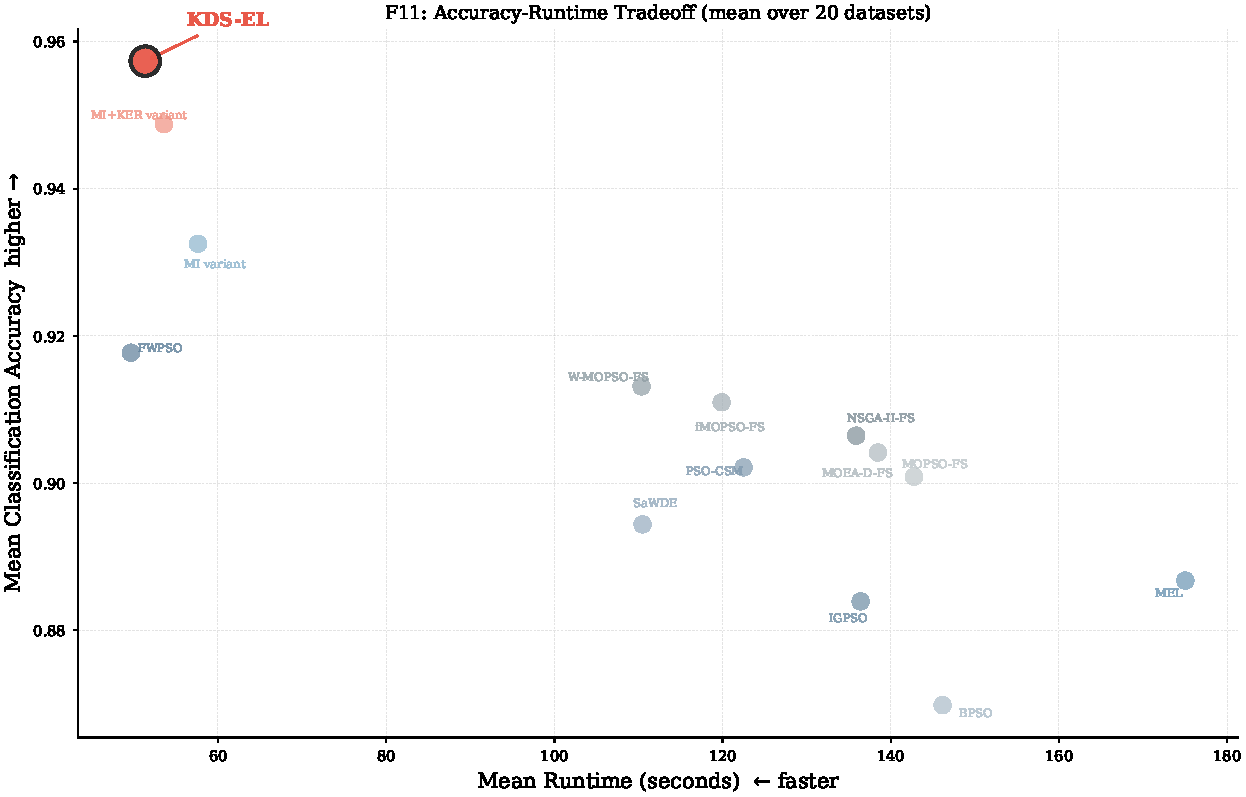
\includegraphics[width=0.85\linewidth]{F11_runtime_scatter.pdf}
\caption{Classification accuracy versus runtime trade-off of the 14 compared methods across the 20 benchmark datasets, illustrating that KDS-EL achieves top classification accuracy with low computational overhead.}
\label{F11}
\end{figure}

KDS-EL achieves an average execution time of \textbf{51.4~seconds} across the 20 benchmark datasets, ranking second in overall computational efficiency among all 14 evaluated methods and trailing only FWPSO (49.7~s) by a marginal 1.7~seconds. Compared with the foundational MEL baseline (175.0~s), KDS-EL achieves an impressive \textbf{3.4$\times$ speedup}. Furthermore, all five multi-objective methods (W-MOPSO-FS, fMOPSO-FS, SaWDE, NSGA-II-FS, MOEA-D-FS, and MOPSO-FS) require between 110.4~s and 142.8~s on average---more than double the runtime of KDS-EL.

The computational scalability of KDS-EL is particularly evident on ultra-high-dimensional datasets:
\begin{itemize}
    \item On \textit{T1D} ($D = 54{,}675$), KDS-EL completes in 118.8~s, running \textbf{2.2$\times$ faster} than PSO-CSM (256.6~s) and SaWDE (216.1~s).
    \item On \textit{BASEHOCK} ($D = 4{,}862, N_{\text{samp}} = 1{,}993$), KDS-EL finishes in 130.1~s, running \textbf{4.7$\times$ faster} than SaWDE (616.0~s) and PSO-CSM (644.7~s).
\end{itemize}

This remarkable efficiency is explained by three synergistic mechanisms:
\begin{enumerate}
    \item \textbf{Substantial reduction in evaluation cost via early sparsity}: In KNN-based wrapper evaluation, distance calculation complexity scales as $O(N_{\text{samp}}^2 \cdot d_{\text{selected}})$. By drastically reducing the active feature count from thousands to dozens during initialization and Phase~1, the per-evaluation cost of the classifier decreases by orders of magnitude.
    \item \textbf{Bounded KER refinement budget}: The KER strategy operates with a bounded elite size ($\mathrm{elite\_k}=3$) and perturbation fraction ($\mathrm{flip\_frac}=0.01$), introducing an incremental complexity of only $O(\mathrm{elite\_k} \cdot \mathrm{flip\_frac} \cdot D)$, which is negligible compared to full population evaluations.
    \item \textbf{Absence of Pareto archive overhead}: Unlike MOFS algorithms that must execute expensive non-dominated sorting ($O(M N^2)$) and crowding-distance calculations at every generation, KDS-EL operates with scalarized dual-phase scheduling, completely eliminating archive maintenance bottlenecks.
\end{enumerate}
Although FWPSO achieves a slightly faster runtime (49.7~s vs.\ 51.4~s) due to early-terminating simulated annealing heuristics, it incurs a substantial \textbf{-3.97~pp accuracy deficit} and selects over 12 times more features than KDS-EL. Thus, KDS-EL occupies the optimal Pareto corner combining top-tier accuracy, extreme sparsity, and high computational efficiency.
